\subsection{Конфигурации планет}

\begin{figure}[h!]
\centering
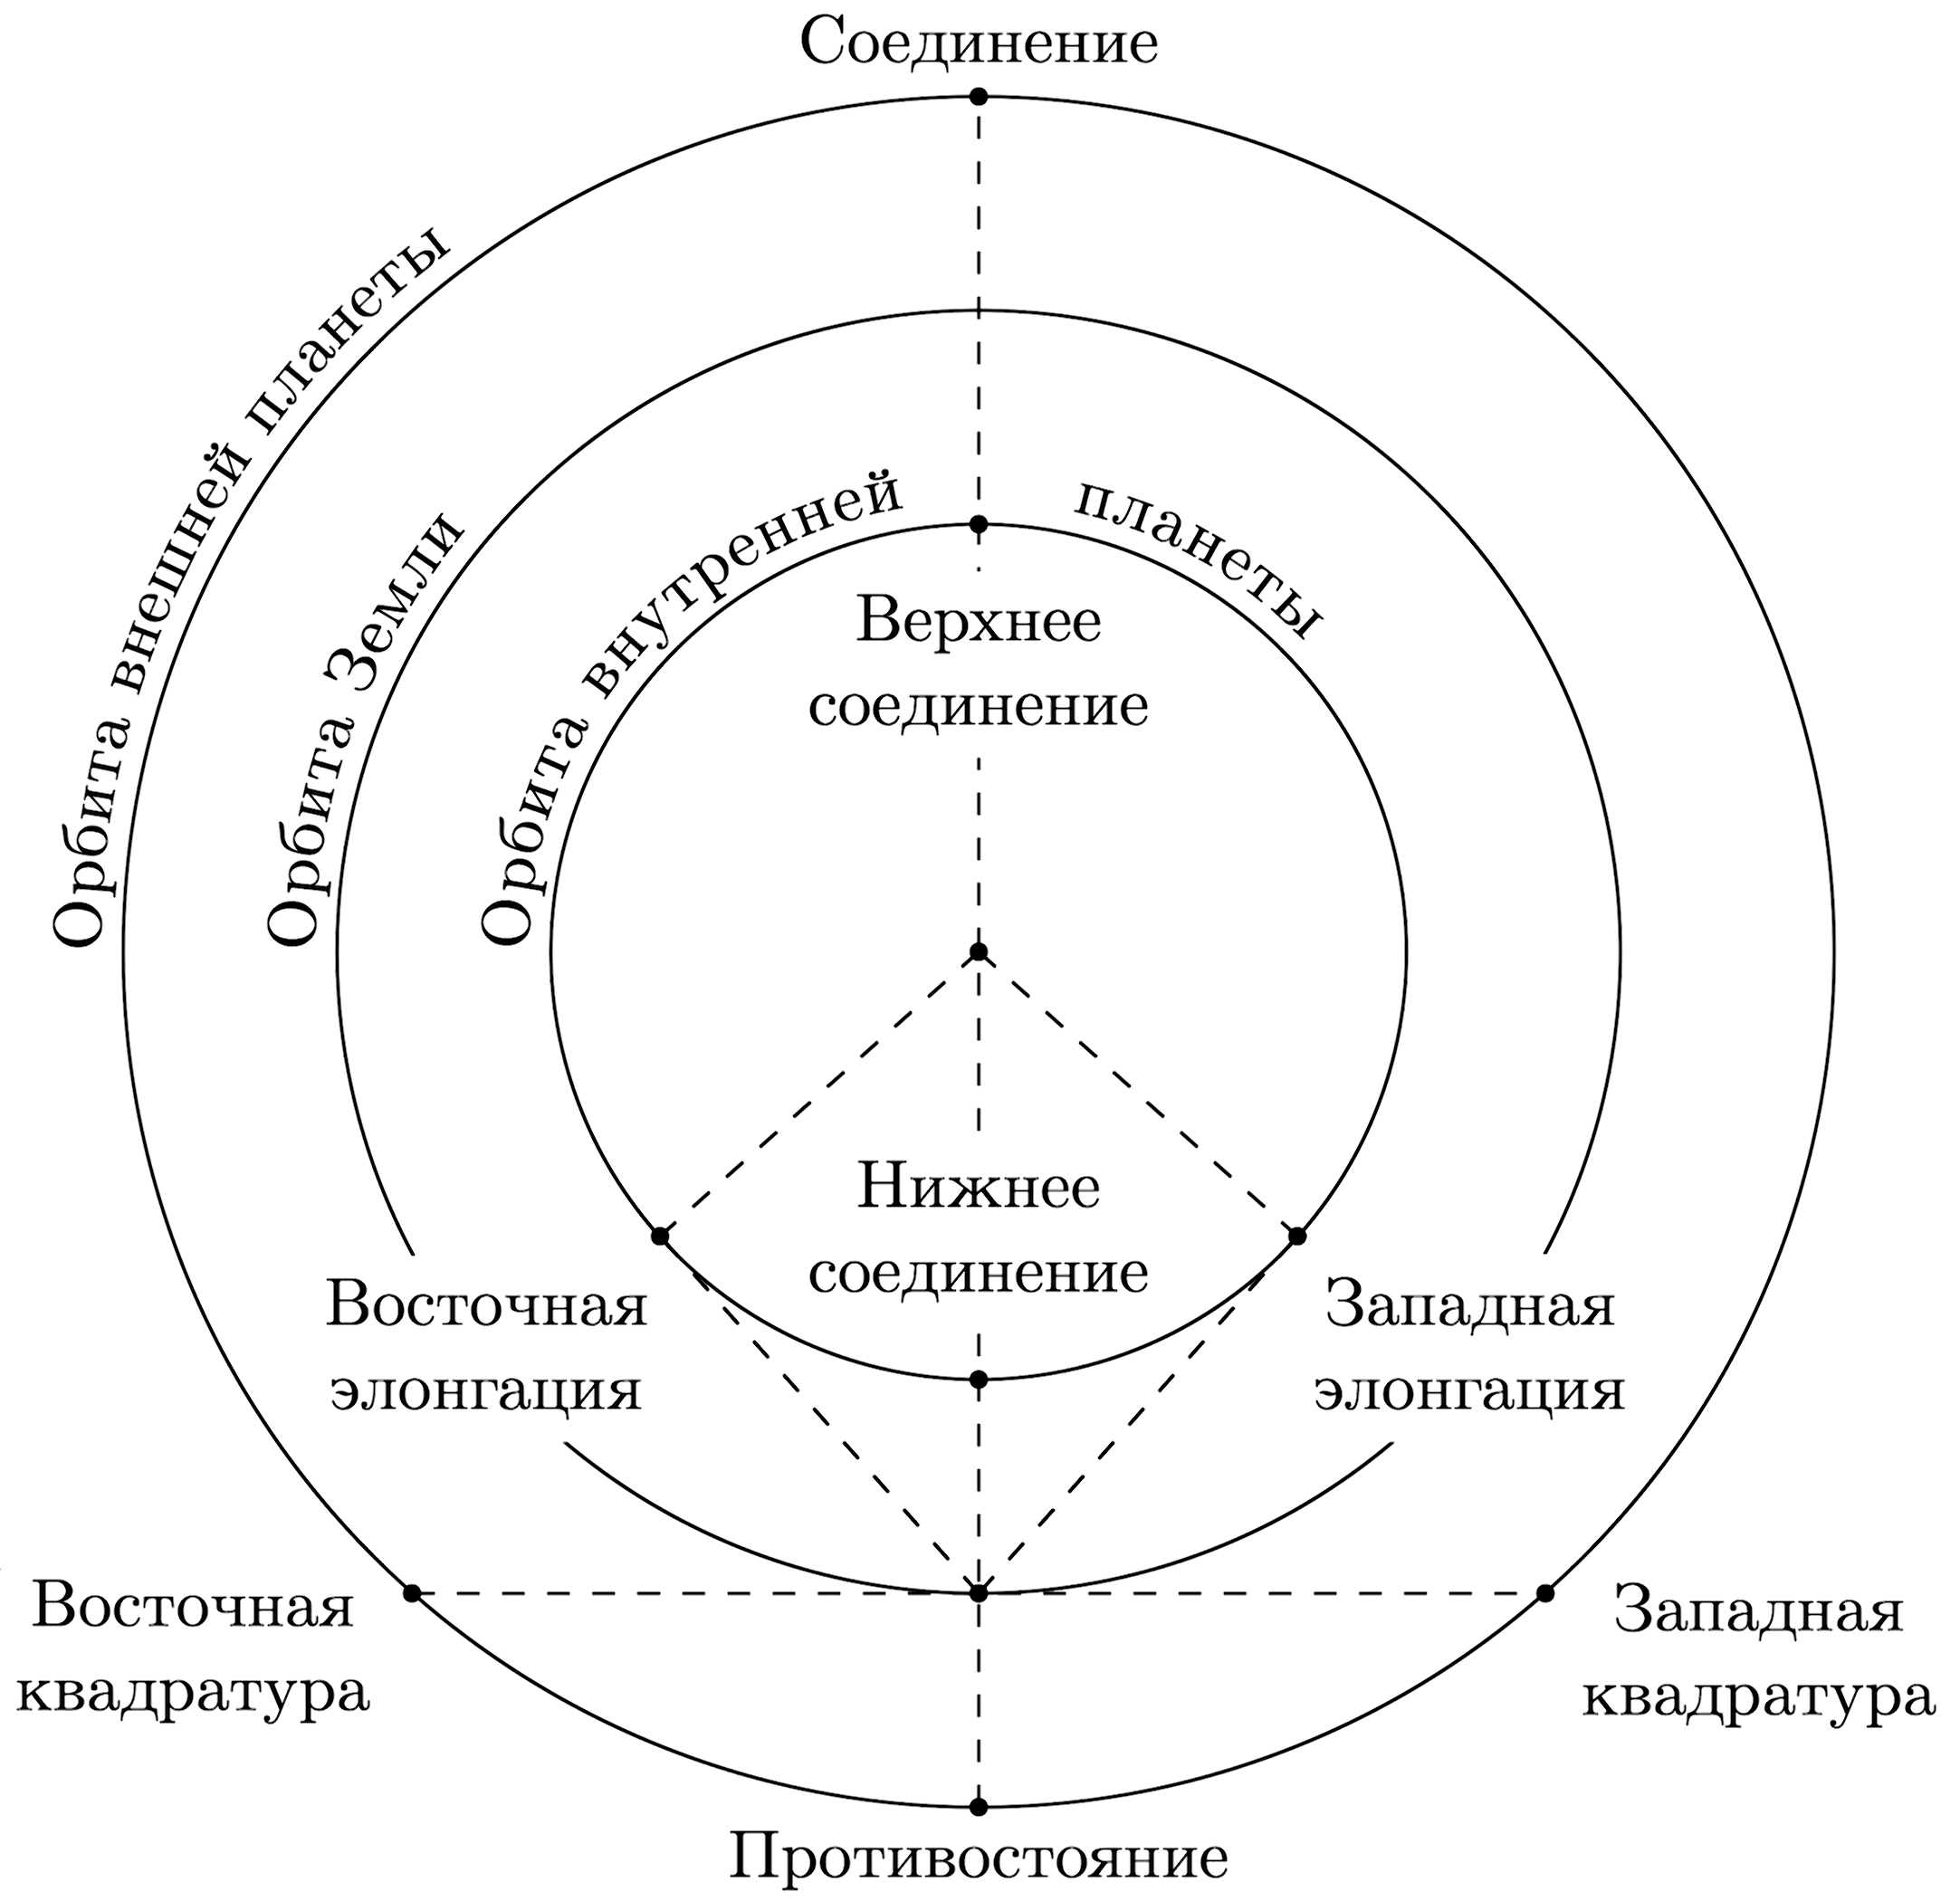
\includegraphics[width = 0.6\textwidth]{planet-config}
\caption{Конфигурации планет}
\end{figure}

{\bfseries Внутренними планетами} называются планеты, 
большая полуось орбиты $a$ которых меньше большой 
полуоси орбиты Земли $a_\oplus$. Отсюда следует, что 
для наблюдателя на Земле {\itshape внутренними} 
планетами являются лишь Венера и Меркурий, остальные 
относятся к {\itshape внешним}. Для таких планет 
выделяют 3 основные конфигурации: {\itshape верхнее 
соединение} (1), {\itshape нижнее соединение} (2) и 
{\itshape максимальная элонгация}. Различают две 
максимальные элонгации --- {\itshape западную} (3) и 
{\itshape восточную} (4), когда планета наблюдается к 
западу и к востоку от Солнца соответственно.

Внутрення планета находится в {\itshape верхнем 
соединении} когда Земля, Солнце и планета лежат на 
одной прямой, при этом планета и Земля располагаются 
по разные стороны от Солнца. Если пренебречь наклоном 
орибит планет к плоскости эклиптики, то для 
наблюдателя на Земле планета находится точно за Солнцем.

{\itshape Нижнее соединение} внутренней планеты 
происходит когда Земля, Солнце и планета, также как и 
в случае верхнего соединения, располагаются на одной 
прямой, но для нижнего соединения планета должна 
находиться между Солнцем и Землей. Если бы орбиты всех 
планет лежали в одной плоскости, тогда в момент каждого 
нижнего соединения внутренней планеты наблюдалось бы 
ее прохождение по диску Солнца для наблюдателя на 
внешней планете.

{\itshape Элонгацией} планеты называется угол Солнце 
-- Земля -- планета, отсюда очевидно, что {\itshape 
максимальная элонгация} внутренней планеты наблюдается 
в момент, когда прямая Земля -- планета является 
касательной к орбите планеты, то есть угол Солнце -- 
планета -- Земля является прямым.\\

{\bfseries Внешними планетами} называются планеты, 
большая полуось орбиты $a$ которых больше большой 
полуоси орбиты Земли $a_\oplus$. Для таких планет 
также существуют 3 основные конфигурации: соединение 
(1), противостояние (2) и квадратура. Квадратура 
бывает западная (3) и восточная (4), в какой именно 
квадратуре находится внешняя планета определяется 
анологично максимальной элонгации.

{\itshape Соединение} внешней планеты, подобно верхнему 
соединению внутренней планеты, наблюдается в момент, 
когда Солнце, Земля и планета находятся на одной прямой, 
при этом Солнце находится между планетой и Землей. В 
этот момент для наблюдателя на внешней планете Земля, 
являясь нижней планетой, наблюдается в верхнем 
соединении.

Аналогично, когда планета, Солнце и Земля располагаются 
на одной прямой, но Солнце и планета лежат по разные 
стороны от Земли, считатется, что внешняя планета 
находится в {\itshape противостоянии}. Земля же находится 
в нижнем соединении для наблюдателя на вненей планете, 
наблюдаемой в противостоянии.

{\itshape Квадратурой} называется конфигурация, когда 
угол между направлениями на планету и Солнце (угол Солнце 
-- Земля -- планета) является прямым. Стоит заметить, 
что для наблюдателя на планете Земля будет наблюдаться 
в максимальной элонгации, причем если планета с Земли 
наблюдалась в восточной квадратуре, тогда Земля будет 
в западной максимальной элонгации и наоборот.
